\documentclass[a4paper]{article}
\usepackage[spanish]{babel}
\usepackage[utf8]{inputenc}
\usepackage{charter}   % tipografia
\usepackage{graphicx}
%\usepackage{makeidx}
\usepackage{paralist} %itemize inline

%\usepackage{float}
%\usepackage{amsmath, amsthm, amssymb}
%\usepackage{amsfonts}
%\usepackage{sectsty}
%\usepackage{charter}
%\usepackage{wrapfig}
%\usepackage{listings}
%\lstset{language=C}


\usepackage{color} % para snipets de codigo coloreados
\usepackage{fancybox}  % para el sbox de los snipets de codigo

\definecolor{litegrey}{gray}{0.94}

% \newenvironment{sidebar}{%
% 	\begin{Sbox}\begin{minipage}{.85\textwidth}}%
% 	{\end{minipage}\end{Sbox}%
% 		\begin{center}\setlength{\fboxsep}{6pt}%
% 		\shadowbox{\TheSbox}\end{center}}
% \newenvironment{warning}{%
% 	\begin{Sbox}\begin{minipage}{.85\textwidth}\sffamily\lite\small\RaggedRight}%
% 	{\end{minipage}\end{Sbox}%
% 		\begin{center}\setlength{\fboxsep}{6pt}%
% 		\colorbox{litegrey}{\TheSbox}\end{center}}

\newenvironment{codesnippet}{%
	\begin{Sbox}\begin{minipage}{\textwidth}\sffamily\small}%
	{\end{minipage}\end{Sbox}%
		\begin{center}%
		\vspace{-0.4cm}\colorbox{litegrey}{\TheSbox}\end{center}\vspace{0.3cm}}



\usepackage{fancyhdr}
\pagestyle{fancy}

%\renewcommand{\chaptermark}[1]{\markboth{#1}{}}
\renewcommand{\sectionmark}[1]{\markright{\thesection\ - #1}}

\fancyhf{}

\fancyhead[LO]{Sección \rightmark} % \thesection\ 
\fancyfoot[LO]{\small{Nombre Apellido, Nombre Apellido, Nombre Apellido}}
\fancyfoot[RO]{\thepage}
\renewcommand{\headrulewidth}{0.5pt}
\renewcommand{\footrulewidth}{0.5pt}
\setlength{\hoffset}{-0.8in}
\setlength{\textwidth}{16cm}
%\setlength{\hoffset}{-1.1cm}
%\setlength{\textwidth}{16cm}
\setlength{\headsep}{0.5cm}
\setlength{\textheight}{25cm}
\setlength{\voffset}{-0.7in}
\setlength{\headwidth}{\textwidth}
\setlength{\headheight}{13.1pt}

\renewcommand{\baselinestretch}{1.1}  % line spacing


% \setcounter{secnumdepth}{2}
\usepackage{underscore}
\usepackage{caratula}
\usepackage{url}


% ******************************************************** %
%              TEMPLATE DE INFORME ORGA2 v0.1              %
% ******************************************************** %
% ******************************************************** %
%                                                          %
% ALGUNOS PAQUETES REQUERIDOS (EN UBUNTU):                 %
% ========================================
%                                                          %
% texlive-latex-base                                       %
% texlive-latex-recommended                                %
% texlive-fonts-recommended                                %
% texlive-latex-extra?                                     %
% texlive-lang-spanish (en ubuntu 13.10)                   %
% ******************************************************** %



\begin{document}


\thispagestyle{empty}
\materia{Organización del Computador II}
\submateria{Segundo Cuatrimestre de 2014}
\titulo{Trabajo Práctico II}
\subtitulo{SIMD}
\integrante{Alejandro Mignanelli}{609/11}{minga_titere@hotmail.com}
\integrante{Franco Negri}{893/13}{franconegri2004@hotmail.com}
\integrante{Federico Suárez}{610/11}{elgeniofederico@gmail.com}

\maketitle
\newpage

\thispagestyle{empty}
\vfill
\begin{abstract}
En el presente trabajo se describe la problemática de procesar información de manera eficiente cuando los mismos requieren:
\begin{enumerate}
\item Transferir grandes volumenes de datos.
\item Realizar las mismas instrucciones sobre un set de datos importante.
\end{enumerate}
\end{abstract}
\thispagestyle{empty}
\vspace{3cm}
\tableofcontents
\newpage

%\normalsize
\newpage

\section{Objetivos generales}

El objetivo de este Trabajo Práctico es mostrar las variaciones en la performance que pueden ocurrir al utilizar instrucciones SIMD en comparación con código C, con diversos grados de optimización realizados por el compilador, cuando se manejan grandes volúmenes de datos que requieren un procesamiento similar.

Para ello se realizarán distintos experimentos sobre cuatro filtros de fotos, Cropflip, Bandas, Sierpinski y Motion Blur, tanto en código assembler, que aproveche las instrucciones SSE brindadas para los procesadores de arquitectura Intel, como en código C compilado con gcc, al que se le aplicarán distintos grados de optimización -O0 (predeterminado), -O1, -O2 y -O3.

El primer filtro, Cropflip, se utilizará para testear performance al utilizar los registros XMM para transferir grandes cantidades de información de un lugar de la RAM a otro.

El segundo, tercer y cuarto filtro, se centrarán en testear la variación de performance al utilizar instrucciones SIMD, no sólo para transferir grandes volúmenes de datos sino también para procesarlos en forma paralela, es decir, realizar diversos cálculos (sumas, multiplicaciones, divisiones) tanto en representación de enteros como punto flotante.

\newpage
\section{Preámbulo}

\subsection{Calidad de las Mediciones}

Antes de comenzar a medir los tiempos de los algoritmos y intentar sacar concluciones de los mismos, debemos plantear un modelo mas o menos claro de como realizar esto mismo.  

Por lo tanto este experimento vamos a ver cómo se ven afectados nuestros algoritmos frente a diversos factores de ruido e interferencias que podrían alterar nuestras mediciones.

Para toda la experimentación se utilizará un procesador Intel Atom, de 2 núcleos a 1.6 GHZ con Hyper-Threading, por lo que la cantidad de núcleos lógicos asciende a 4. Por otro lado, para que las pruebas sean mas concisas y exactas, se deshabilitó el scaling dinamico del CPU, ya que esto podría resultar en mediciones inconsistentes. 

El software utilizado será Ubuntu 14.04, GCC 4.8.2, y nasm 2.10.09.

Para ver como se veían afectados los resultados procedemos a tomar 1000 mediciones para cada una de las versiones del cropflip, tanto con 4 loops corriendo en paralelo (uno por cada core logico) como sin los mismos.

A los datos obtenidos tomamos el promedio para obtener un valor aproximado de cuanto tarda en correr cada uno de los algoritmos y calculamos el desvío estandar para ver cuanto se desvían de la media las mediciones. Los resultados pueden verse en este grafico:

\begin{center}
  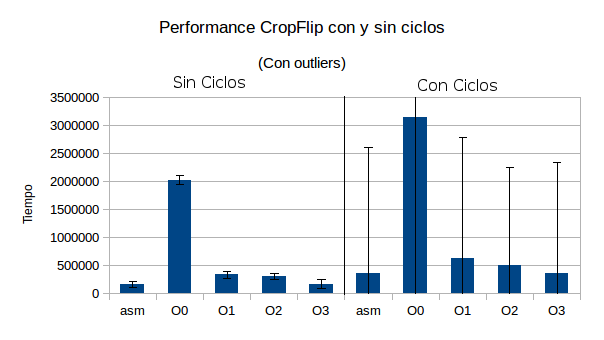
\includegraphics[scale=0.66]{Graficos1.4/1.3/perConOut.png}
\end{center}

Vemos que con loops, los datos se dispersan de una manera incontrolable, a tal punto que es imposible sacar ninguna conclusión de los mismos. Ahora para intentar obtener un desvío estandar un poco mejor, consideramos los $200$ valores más grandes y los $200$ valores más chicos como outliers y los quitamos tanto del promedio como del desvío estandar.

Volviendo a graficar:

\begin{center}
  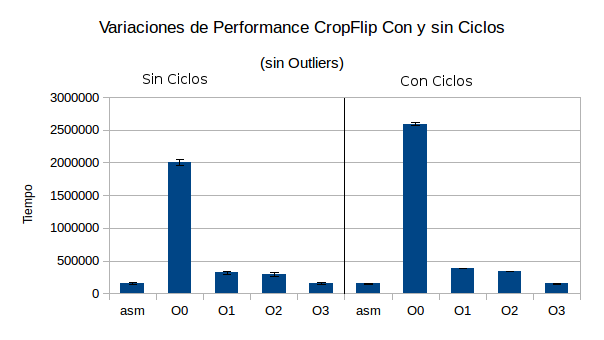
\includegraphics[scale=0.66]{Graficos1.4/1.3/perSinOut.png}
\end{center}

De esta manera logramos obtener valores mucho mas razonables para el desvío estandar en ambos casos.

De este último gráfico además podemos observar que los loops afectan de manera diferente a los algoritmos, el código de C sin optimizar aumenta su tiempo de ejecución en un 25 \%, mientras que el código de assambler no varía en lo mas mínimo.

Finalmente, para intentar mantener el desvío estandar en un valor lo mas pequeño posible y para evitar este aumento no proporcional en el tiempo de ejecución de los algoritmos, se determina que para cada experimento en el presente informe, se tomaran 1000 mediciones sin loops corriendo en simultaneo y quitando los outliers antes mencionados.

\newpage

\section{Experimentación}

\subsection{Desensamblado de código C y Optimización}

Ahora en esta sección procedemos a analizar el código de generado por GCC para intentar dilucidar como genera los binarios. Para eso realizamos un objdump del codigo del Cropflip sin ningun grado de optimización.

Este algoritmo básicamente mueve datos de un lugar de la RAM a otros, sin afectar mayormente los valores de la imagen.

Al desensamblar el código podemos observar, primero que nada, que GCC guarda todos los parámetros en la pila y además está escribiendo en memoria todas las variables locales utilizadas, lo cual es innecesario ya que pueden ser almacenadas en registros.

También puede observarse que el compilador genera codigo con saltos incondicionales, lo que puede sugerir que intenta sacar provecho al sistema de predicción de saltos.

Ademas GCC genera, luego de la función, un montón de secciones que comienzan con debug_xxx. Estas secciones segun lo que encontramos en internet, sirven para ser interpretadas por GDB u otros debuggers y ayudar al programador en el momento de testeo.

Como ya dijimos, el código podría optimizarse para no realizar tantos accesos a memoria innecesarios guardando variables locales por ejemplo en registros, lo cual disminuiría el tiempo de ejecución.

Ahora procedemos a compilar el código utilizando el flag -O1, y nuevamente realizamos un objdump para observar los cambios en el codigo. Se observa que ahora el mismo solo realiza los accesos a memoria mínimos indispensables, utilizando los registros para guardar los datos. Además el código es más compacto, y resulta mas claro de leer. Asimismo precalcula los valores que serán utilizados muchas veces, lo que seguramente aumenta la performance, principalmente en casos de instancias grandes.

Los otros flags de optimización disponibles en GCC son -O2, -O3, -Og, -Os, -Ofast. También podemos encontrar los flags -msse, -msse2, -msse3, -mmmx, -m3dnow, pero al intentar compilar con varios de ellos vimos que el compilador no utilizó instrucciones SIMD.

De las muchas optimizaciones que el compilador puede realizar, tomamos tres para ejemplifiacar: -foptimize-sibling-calls, -finline-small-functions, -fmerge-constants.

La optimizacion -foptimize-sibling-calls, sirve para optimizar las funciones con recurcion a la cola.Por otra parte -finline-small-functions integra funciones a las funciones que las llaman cuando el cuerpo de la función es menor que la cantidad de instrucciones necesarias para llararla, resultando en un codigo de menor tamaño. Por ultimo -fmerge-constants intenta mergear constantes identicas entre las distintas unidades de compilación.

\newpage

\section{Cropflip}

\subsection{Diferencias de performance en Cropflip}
Para este experimento se medirán las performances tanto de nuestro algoritmo en assembler, implementado para sacar provecho de las instrucciones SSE de Intel, como una versión alternativa implementada en C aplicando diversos grados de optimización a cargo del compilador.

El algoritmo de Cropflip en assembler es muy sencillo. Simplemente movemos 128-bits de la imagen a un xmm y de allí al destino, que previamente ha sido seteado para colocar los bits en el lugar correcto. De esta manera, podremos mover de una sola vez, 16 bytes, lo que corresponde a 4 píxels de la imagen.

Dado que la cantidad de columnas es siempre múltiplo de 4, o sea, siempre tenemos 4 bytes para tomar, no es necesario chequear otros casos borde.

Como acordamos en el apartado de calidad de mediciones, tomamos 1000 muestras, quitamos los outliers y calculamos el promedio y el desvío estandar:

\begin{figure}[h!]
  \begin{center}
	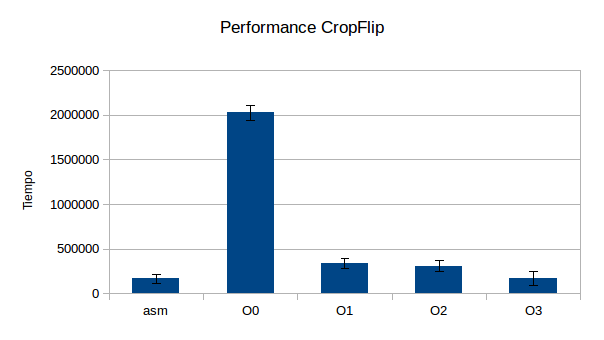
\includegraphics[scale=0.66]{Graficos1.4/crop/per.jpg}
	\label{nombreparareferenciar5}
  \end{center}
\end{figure}

\subsubsection{Resultados}

En el gráfico puede verse que la version SIMD del algoritmo de cropflip  y la version C con mayor grado de optimización son muy parecidas en cuanto a performance, aunque el desvío estandar del codigo C es levemente mayor a la del primero ($52367$ del codigo en asambler contra $75973$ del codigo en C). Por otro lado, el codigo desarrollado en ensamblador tiene una mayor performance comparado con los codigos en C con optimizaciones O1 y O2, y en comparacion con el codigo generado con el flag -O0 el codigo asm es 8 veces más rápido.

\subsubsection{Conclusiones}
Una de las razones por las que el código optimizado a nivel 3 puede obtener tan buenos resultados como los de SIMD, es que al optimizar con este nivel se activa un flag (-fipa-cp-clone) que permite hacer algo llamado interprocedural constant propagation, que según entendemos intenta paralelizar el código, o alguna otra optimización del codigo que lo hace extremadamente performante incluso sin utilizar SIMD. Aún así, prestándole más atención al desvío estándar, pareciera que este codigo tiene una mayor variabilidad que nuestro codigo en asambler, asi que igualmente, nuestro código pareciera tener alguna ventaja sobre el codigo generado en C.

\newpage

\subsection{cpu vs. bus de memoria en Cropflip}

En este experimento lo que hicimos fue agregar instrucciones aritméticas por un lado y instrucciones de lectura-escritura por otro para ver como influía esto en el tiempo de ejecución del codigo en assambler.

Para eso agregamos $4$, $8$ y $16$ instrucciones de lectura-escritura por un lado y $4$, $8$ y $16$ instrucciones aritméticas entre registros en el loop principal del código assambler y comparamos las performance entre sí y con la versión original.

Lo que obtuvimos puede verse aquí:

  \begin{center}
  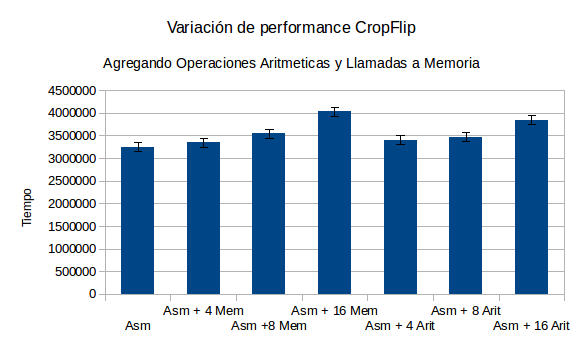
\includegraphics[scale=0.66]{Graficos1.5/crop/per.png}
  \end{center}


\subsubsection{Resultados}
Lo que vemos en el gráfico es que al agregar tanto operaciones aritméticas como operaciones de memoria, el tiempo aumenta. Por otro lado, se observa que agregar n accesos a memoria (con n= $4$, $8$ o $16$), tarda más tiempo que agregar las mismas n operaciones aritméticas.

\subsubsection{Conclusiones}

Lo obtenido en los resultados era de esperar ya que es sabido que el cuello de botella del modelo Bon-Newman y en las arquitecturas modernas, ocurre en el momento de ir a buscar datos a memoria, de allí que sea necesario agregar distintas cachés para intentar que la disminución de la performance sea menor. En otras palabras, de aquí se puede comprobar de manera empírica que para el procesador es más costoso acceder a memoria que realizar operaciones lógicas. 

\newpage
\section{Sierpinski}

\subsection{Idea general del algoritmo}

Comenzaremos esta sección describiendo la idea tras el algoritmo de Sierpinski. En este caso, el algoritmo ya es un poco más complejo. Necesitamos calcular para cada píxel un coeficiente diferente, que dependerá de la posición $(i,j)$ de cada píxel.

Luego para poder paralelizar de alguna manera el algoritmo y sacar provecho a los registros xmm, es necesario calcular 4 coeficientes a la vez y multiplicárselos a sus respectivos píxels.

Luego la idea del algoritmo implementado en ensamblador será la siguiente:

Al comenzar el ciclo, leemos 4 píxels y los guardamos en un registro xmm. Luego, calculamos el coeficiente para cada píxel de forma paralela como se muestra en el dibujo.

\begin{center}
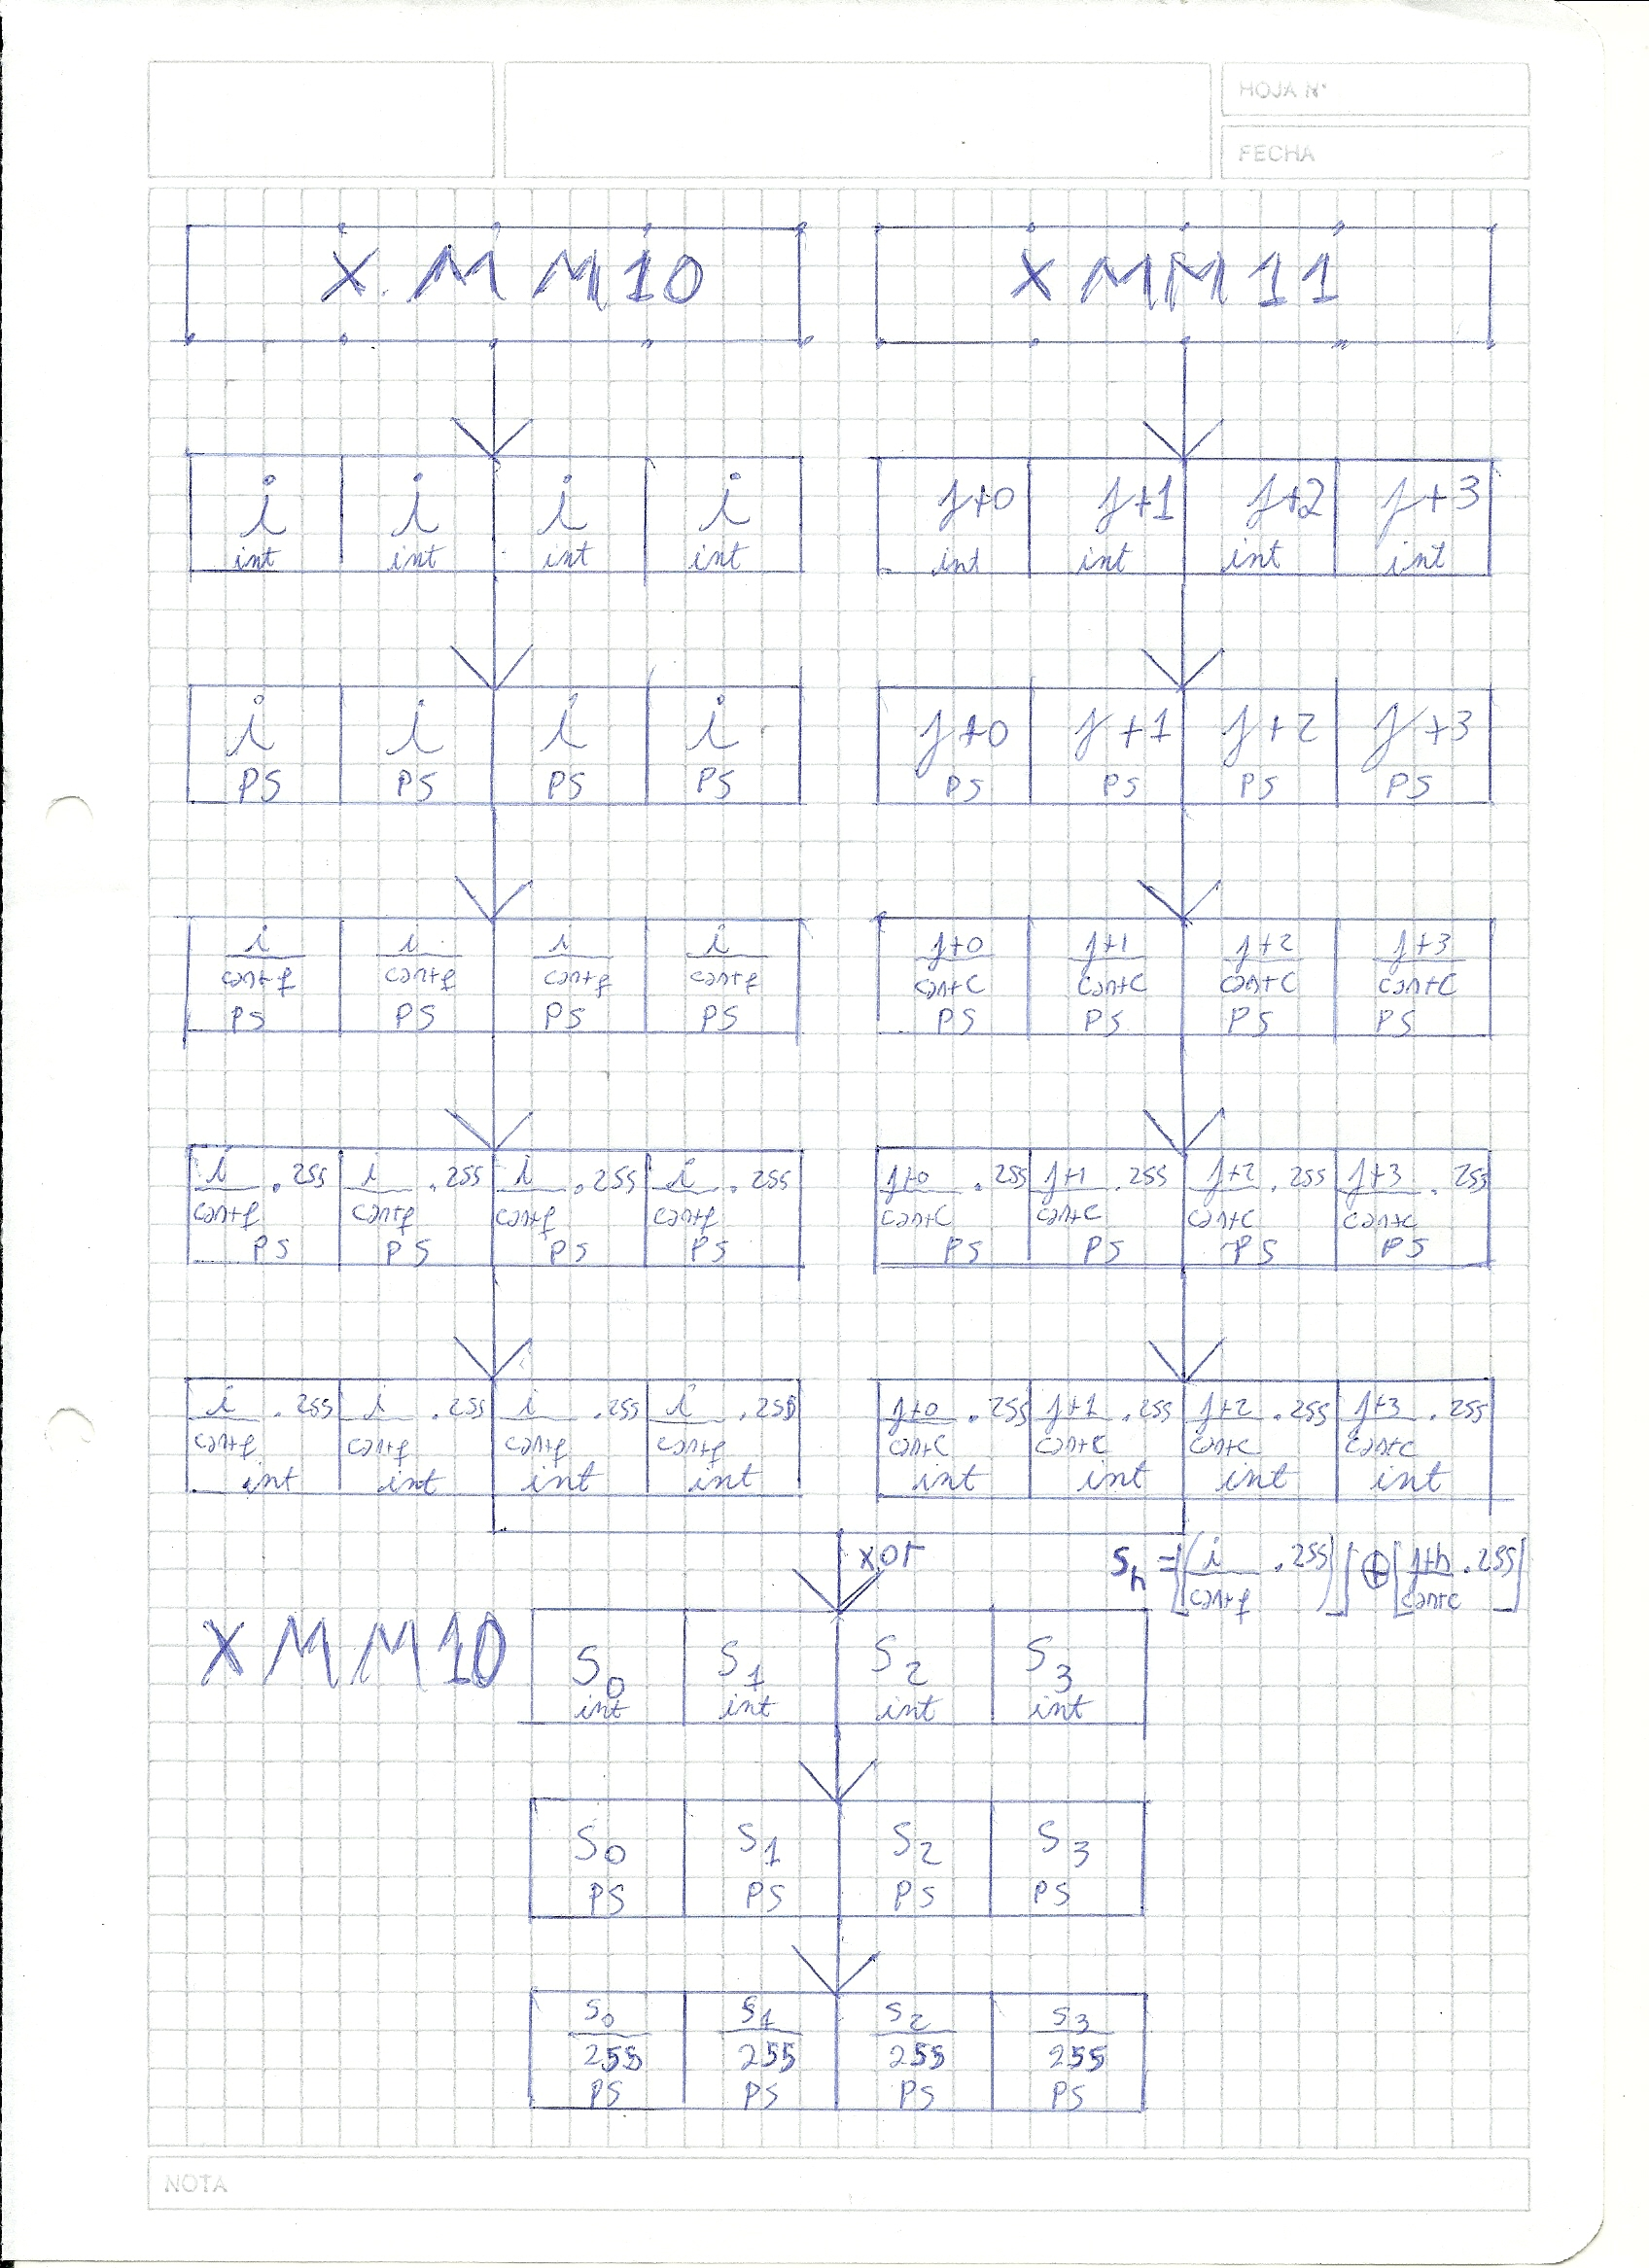
\includegraphics[scale=0.75]{Dibujos/S1.jpg}
\end{center}

Una vez obtenidos los coeficientes, sólo nos resta multiplicar a cada uno por el píxel correspondiente. Como debemos multiplicar dicho coeficiente por cada byte de cada píxel, primero deberemos desempaquetar los datos de tal manera que nos queden 4 registros xmm, uno para cada píxel, que cada uno contenga todos los bytes del píxel asociado en el orden original. A continuación, nos toca convertir todo a punto flotante para poder realizar la multiplicación. Además necesitaremos brodcastear el coeficiente de cada píxel en un registro xmm para así efectivamente multiplicarlo por cada componente del píxel. Después de terminar con las multiplicaciones, convertimos a entero nuevamente y empaquetamos todo para finalmente moverlo al destino.

\subsection{Diferencias de performance en Sierpinski}

Los resultados comparativos de performance para este algoritmo comparado con uno desarrollado en C fueron los siguientes:

  \begin{center}
  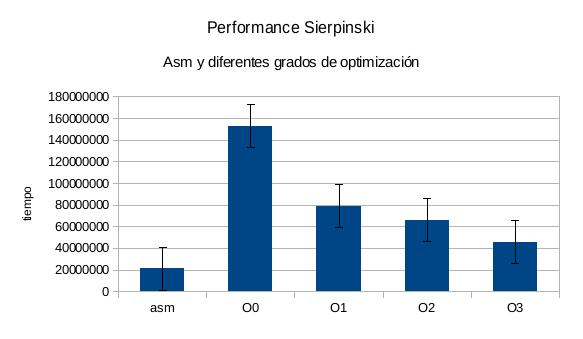
\includegraphics[scale=0.66]{Graficos1.4/sie/per.jpg}
  \end{center}

\subsubsection{Resultados}
En el gráfico puede notarse que el codigo en ensamblador es aproximadamente dos veces más rápido que la versión de C optimizada con O3, más de tres veces más rápido que el optimizado con O2 y O1 y más de 7 veces más veloz que el codigo C sin optimizar. El desvío estándar en este caso es tan pequeño que casi no puede verse en el gráfico (Dos ordenes de magnitud menor que el promedio en todos los casos).
\subsubsection{Conclusiones}

De lo que podemos observar, concluímos que en este caso, paralelizar los datos y operar sobre ellos resulta en un incremento de la performance incluso superior al codigo en C con mayor grado de optimización. Esto se ve respaldado por los bajos desvíos estandards, ya que le dan mayor confiabilidad a nuestros resultados.

\newpage
\subsection{CPU vs. Bus de memoria en Sierpinski}

Realizamos el mismo experimento que hicimos para cropflip, es decir, agregamos instrucciones aritméticas y de lectura escritura al código assambler para medir su desempeño.

Tomando el promedio y graficando los valores obtenidos:

  \begin{center}
  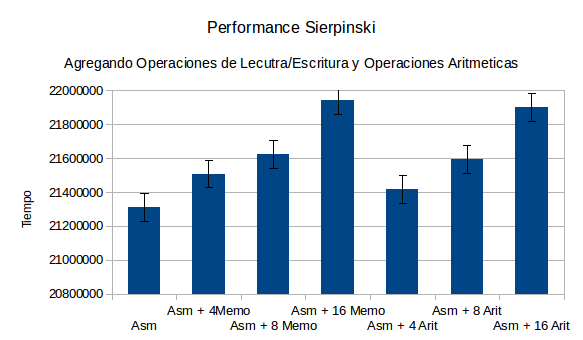
\includegraphics[scale=0.66]{Graficos1.5/sie/per.png}
  \end{center}

\subsubsection{Resultados}
Se observa que al agregar operaciones, tanto aritméticas como de lectura-escritura, el tiempo de ejecución aumenta. Tambien, como en el caso anterior, agregar un numero de operaciones aritméticas y agregar el mismo número de operaciones de lectura-escritura, estas últimas repercuten en un mayor tiempo de ejecución.

\subsubsection{Conclusiones}

Nuevamente podemos llegar a la misma conclusión que antes, el cuello de botella se encuentra en el tiempo que el procesador tarda en buscar datos a memoria. Incluso implementando técnicas abanzadas como caché y ejecución fuera de orden, la caida en performance es notable.

Tal vez en este caso la diferencia es menos marcada porque ya se le estaba dando un uso exaustivo a la ALU y agregar más operaciones aritméticas resulta mas costoso aquí que en el caso del cropflip, donde la ALU no era mayormente utilizada.

\newpage
\section{Bandas}
\subsection{Idea general del algoritmo}
Para el algoritmo de bandas se nos presenta otro desafío: debemos tomar los tres colores de la imagen $(r,g,b)$, sumarlos, y luego comparar cada uno de ellos para ver si se encuentra en un rango determinado.

Dado este problema tan particular buscamos en el manual de intel aluna instrucción que nos pueda ayudar a realizar esto de manera facil. Descubrimos que tenemos a dispocición la instrucción PADD que suma de manera horizontal como se muestra en el siguiente grafico:

\begin{center}
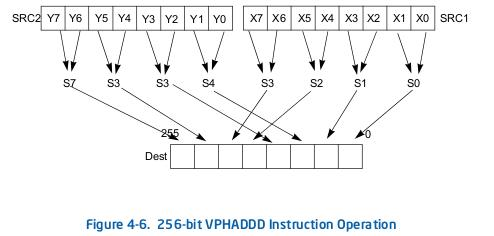
\includegraphics[scale=0.66]{Dibujos/SH.jpg}
\end{center}

Si bien en el dibujo se muestra la instruccion para un registro de 256 bits, existe una que funciona de manera similar para un XMM de 128 bits, que es la que utilizaremos nosotros.

Teniendo esto en cuenta, la idea del algoritmo es la siguiente:

Como primer paso, leemos los 4 píxels y los guardamos en un xmm. Luego, desempaquetamos los datos de byte a word para poder realizar la suma de las componentes de cada píxel sin salirnos de la representación. La suma se hace a través de dos instrucciones de la suma horizontal antes mencionada, de tal manera que nos quedan los $b$ de cada píxel en las cuatro words de la parte baja de un xmm. A continuación realizamos unas comparaciones utilizando máscaras predefinidas para determinar el valor que tendrá cada píxel en cada una de sus componentes.Para asignar dicho valor, se tomará un xmm que viene seteado en 255 de a words en la parte baja, en donde se irá guardando el resultado. Luego, por como fue implementado el algoritmo, y tomando como p un word del xmm que viene seteado con 255 en la parte baja, y como v el word correspondiente que tiene la suma de r+g+b, cada word independientemente del resto seguirá el siguiente esquema:

\begin{center}
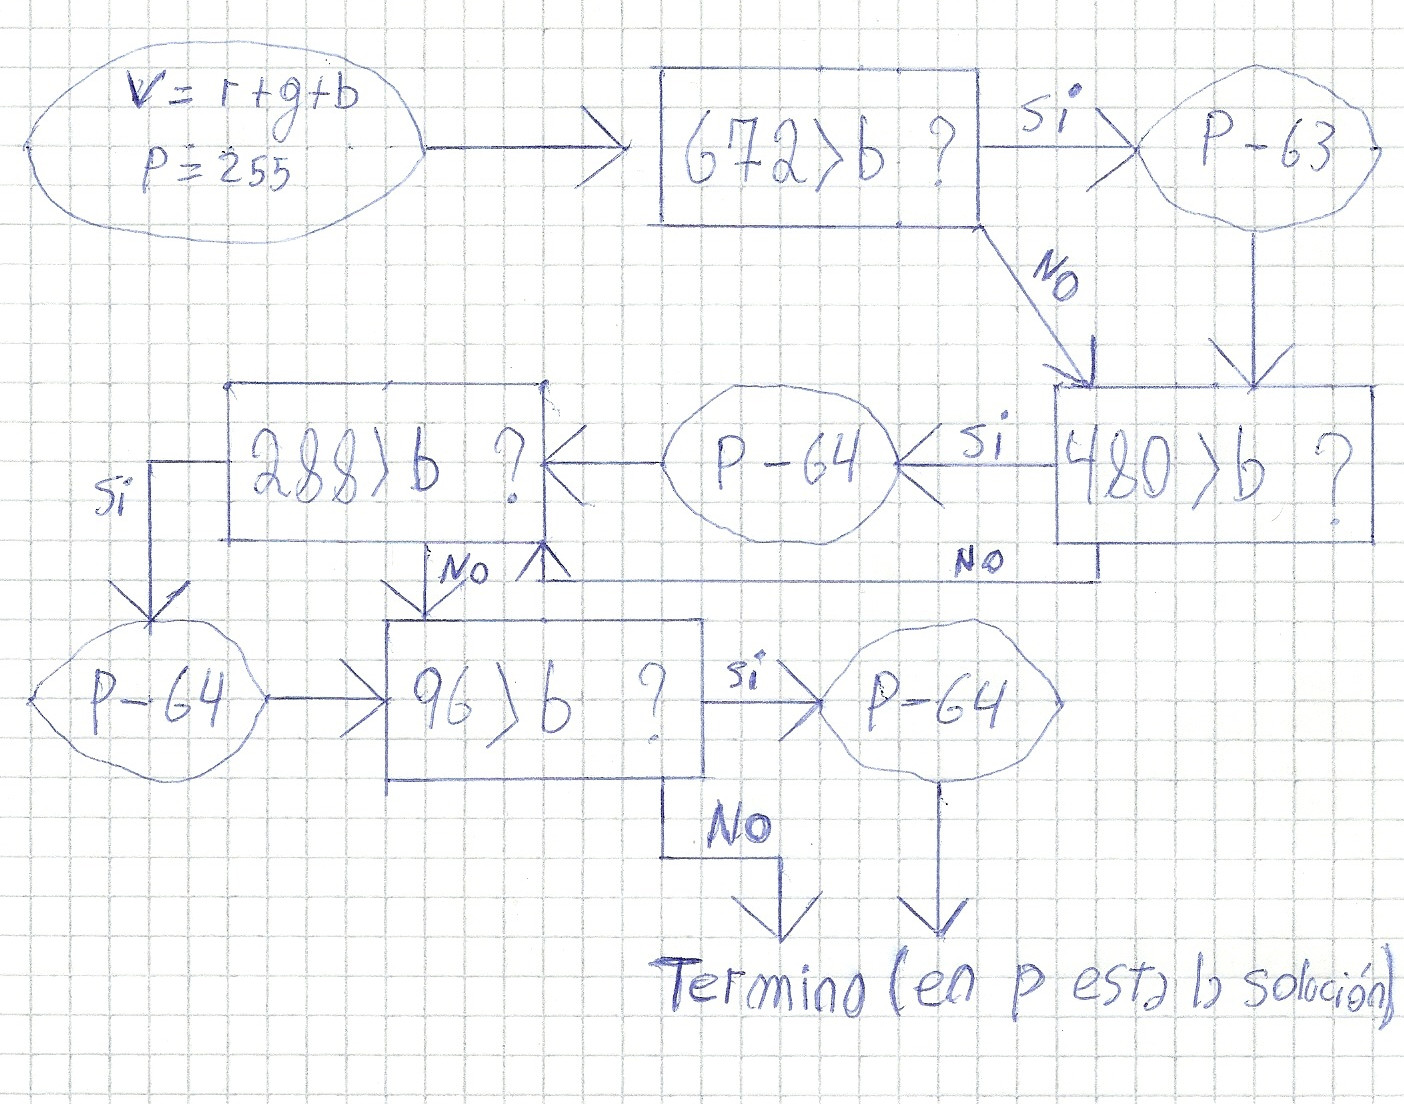
\includegraphics[scale=0.66]{Dibujos/B1.jpg}
\end{center}


 Después de realizadas estas comparaciones, nos queda en las word de la parte baja del xmm que guardaba el resultado, los 4 valores que se asignarán a cada componente de cada píxel. Luego, empaquetamos estos valores pasandolos de word a byte y aplicamos un shuffle que los deja en el los lugares que corresponden para finalmente copiarlos al destino. 

\subsection{Diferencias de performance en Bandas}

Realizamos un testeo similar para este algoritmo y obtenemos lo siguiente:

\newpage

  \begin{center}
  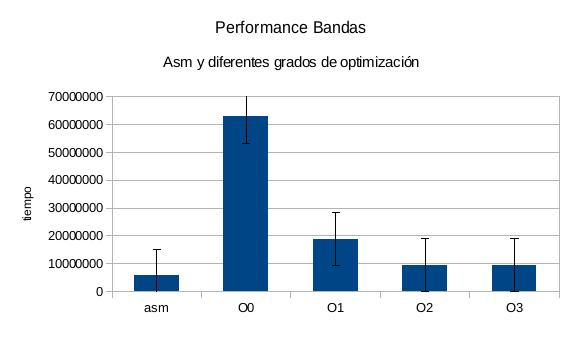
\includegraphics[scale=0.66]{Graficos1.4/ban/per.jpg}
  \end{center}

\subsubsection{Resultados}
Se puede observar que el algoritmo en asm con SIMD tarda casi la mitad de tiempo que C con optimización O3 y O2. Tambien es aproximadamente tres veces más veloz que la optimización O1, y 7 veces más rápido que O0.

El desvío estandar es muy pequeño.

\subsubsection{Conclusiones}

Nuevamente podemos concluir que resulta ventajoso utilizar instrucciones vectoriales para realizar cálculos paralelizados sobre un gran volumen de datos.

\newpage
\subsection{Saltos condicionales}

En este experimento veremos como afectan los saltos condicionales a la performance del codigo C compilado con -O1. Para ello lo que haremos es quitar los IFs del código dejando solo una banda, luego medir la performance y compararla con la versión con saltos.


  \begin{center}
  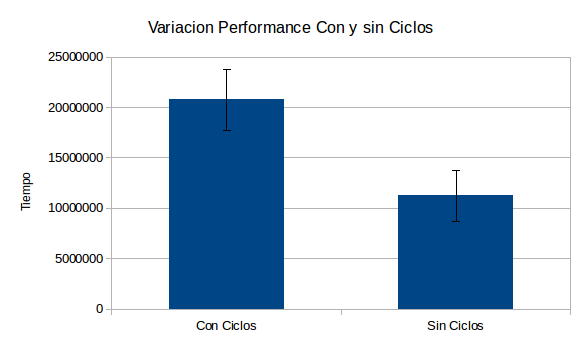
\includegraphics[scale=0.66]{Graficos3.1/per.png}
  \end{center}

\subsubsection{Resultados}
En el gráfico puede observarse una gran diferencia entre el código que tiene saltos condicionales y el código que no los tiene. El desvío estandar también es levemente diferente, $3051803$ del código con saltos a $2504091$ sin los mismos.

\subsubsection{Conclusiones}

La variación de tiempos ocurre posiblemente debido a que en el caso del código con saltos, el procesador para no perder tiempo esperando que la condición sea resuelta y poder seguir ejecutando fuera de orden, toma todas las posibles ramas de la ejecución. Esto sin duda causará que el procesador este más ocupado realizando cálculos en todas las ramas y aumente el tiempo de ejecución. Esto también explicaría por que los datos estan mas dispersos en el caso del codigo con saltos, ya que el CPU se vuelve menos predecible.

\newpage
\section{Motion Blur}
\subsection{Idea general del algoritmo}
La idea de este algoritmo es, por cada píxel del destino se deben tomar 5 píxels de la entrada, se multiplica cada uno de los colores por $0.2$ y luego se los suma. Lo que realmente haremos en el algoritmo será primero hacer la suma y luego multiplicar por $0.2$ ya que esto requiere menos registros XMM.

Una idea general de cómo funciona el algoritmo en assembler es la siguiente:

Al comenzar el ciclo, esta vez no sólo leeremos 4 píxels, sino que también leeremos píxeles de las filas vecinas ya que para procesar un píxel $(i,j)$ necesitaremos además los 4 píxels de las filas $i-2$, $i-1$, $i+1$ e $i+2$ en las columnas $j-2$, $j-1$, $j$, $j+1$ y $j+2$, respectivamente. Debido a esto debemos tener cuidado de tomar correctamente los casos borde y no aplicar motion blur donde no corresponde.

Gráficamente, tomaremos los píxeles y sus vecinos de la siguiente forma(esto es un ejemplo en un caso donde recien se toman los primeros cuatro píxeles a modificarse):

\begin{center}
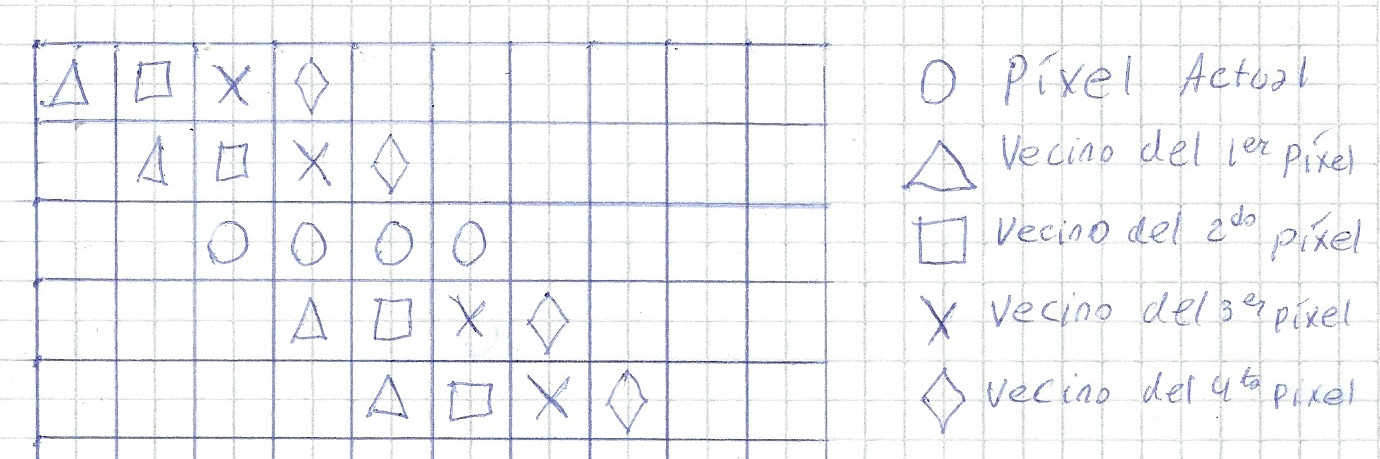
\includegraphics[scale=0.66]{Dibujos/MB1.jpg}
\end{center}

Luego, desempaquetamos todo a word para realizar la sumas sin irnos de la representación.Teniendo todo en muchos xmm de a words, separados en parte alta y baja, se empezarán a sumar lo correspondiente a cada píxel(el original y sus vecinos) con sumas verticales, que funcionan de la siguiente manera(la siguiente imagen es una suma vertical de a words):

\begin{center}
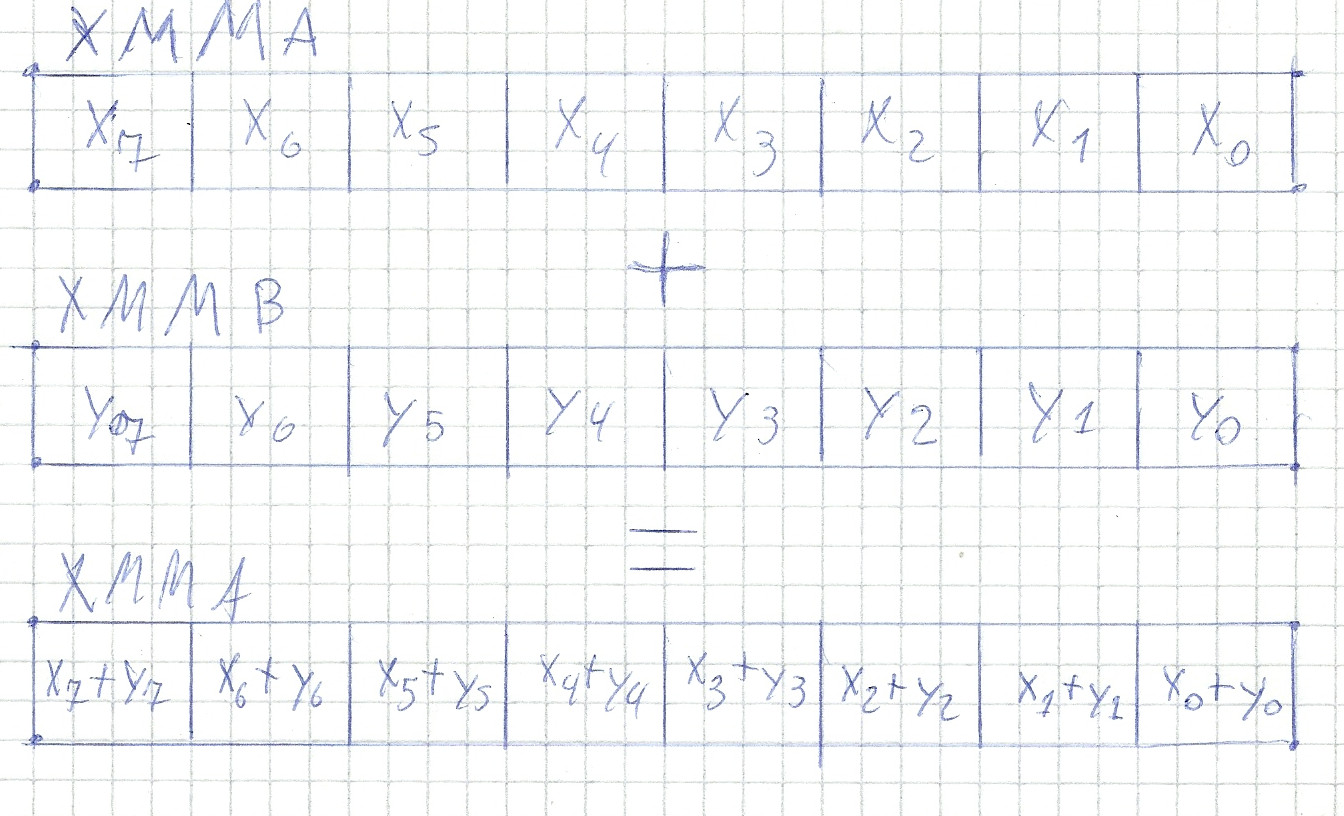
\includegraphics[width=0.9\textwidth]{Dibujos/sv.jpg}
\end{center}

Cuando ya hemos sumado lo que necesitamos, desempaquetamos nuevamente pero ahora a dword para poder convertir a punto flotante y así luego multiplicar por $0.2$. Una vez realizada la multiplicación, convertimos a entero nuevamente y empaquetamos todo de dword a word, y de word a byte. Finalmente, copiamos los 4 píxels procesados al destino. Además de todo esto, cada vez que terminamos de recorrer una fila, ponemos en negro los siguientes 4 píxeles, y las dos primeras y últimas filas las ponemos en negro aparte, fuera del ciclo.

\subsection{Diferencias de performance en Motion Blur}

Al realizar el testing se obtuvieron los siguientes resultados:

%\newpage

\begin{figure}[h!]
  \begin{center}
  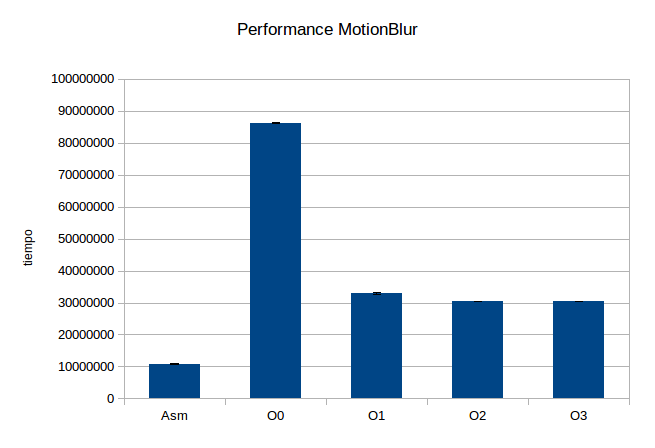
\includegraphics[scale=0.66]{Graficos1.4/mbl/per.jpg}
  \label{nombreparareferenciar11}
  \end{center}
\end{figure}

\subsubsection{Resultados}
Se aprecia en el gráfico que el código ASM con SIMD tiene un promedio de tiempo de ejecucion aproximadamente tres veces menor a la mayor optimización de C, y varias veces menor que O0. También se observa que O1, como O2 y O3 dan promedios de tiempo muy parecidos. Las varianzas son similares y muy pequeñas.

\subsubsection{Conclusiones}

En este caso podemos concluir nuevamente que la opcion en assambler es mejor que la opción en C que no utiliza operaciones vectoriales, incluso con el mayor grado de optimización es posible lograr una mejora del 66 \% aproximadamente.

\newpage
\section{Conclusiones y trabajo futuro}

Como primera conclución de este trabajo practico podemos decir la gran ventaja que reperesenta la utilización de operaciones vectoriales a la hora de realizar operaciones paralelizables sobre un gran volumen de datos. También podemos concluir que esto no resulta de la misma manera en el caso de transferir información de un lugar de la memoria RAM a otro, ahí, la opción de implementar código C optimizado es tan buena como la de implementarlo con SIMD, con la ventaja de que en C el código es más facilmente mantenible y claro.

Otras concluciones son, que la comprobación de manera empirica que el acceso a RAM presenta una mayor caída de performance que las operaciones aritméticas. Y que el branch prediction tambien representa una mayor caída en la performance, por lo que utilizar otras opciones que no requieran saltos condicionales es una buena opción de mejorar los tiempos de un algoritmo dado.

Como trabajo futuro, una idea interesante a desarollar, podría ser construir o plantear un compilador de C que tome la mejor parte de los compiladores actuales, esto es, las diversas optimizaciones que realiza, y las integre con SIMD. De esta manera se podría, en teoría, obtener mejores resultados que los aquí mostrados.

\end{document}

